%
% 6.857 homework template
%
% NOTE:
% Be sure to define your team members with the \team command
% Be sure to define the problem set with the \ps command
% Be sure to use the \answer command for each of your answers
\documentclass[11pt]{article}


%\pagestyle{headings}
\usepackage[dvips]{color}
\usepackage{amsfonts}
\usepackage{amssymb}
\usepackage{amsmath}
\usepackage{latexsym}
\usepackage{fancyvrb}
\usepackage{listings}
\usepackage{color}

\definecolor{mygreen}{rgb}{0,0.6,0}
\definecolor{mygray}{rgb}{0.5,0.5,0.5}
\definecolor{mymauve}{rgb}{0.58,0,0.82}
\setlength{\parskip}{1pc}
\setlength{\parindent}{1pt}
\setlength{\topmargin}{-3pc}
\setlength{\textheight}{9.0in}
\setlength{\oddsidemargin}{1pc}
\setlength{\evensidemargin}{1pc}
\setlength{\textwidth}{6in}

\usepackage{graphicx}
\usepackage{enumitem}
\usepackage{placeins}
\setdescription{leftmargin=\parindent,labelindent=\parindent}

\begin{document}

\begin{titlepage}



% Title
{ \huge \bfseries Placr\\[0.4cm] }
% Author and supervisor
\begin{minipage}{0.4\textwidth}
Ryan Cheu \\ryancheu@mit.edu\\\\
David Kang \\wkang@mit.edu\\\\
Ben Zinberg \\bzinberg@mit.edu\\
\end{minipage}



\vfill

% Bottom of the page
{\large \today}

\end{titlepage}
\newpage


\LARGE{\textbf{1 Introduction}}

\normalsize


This report outlines the design for Placr, a system for controlling the placement of virtual machines (VMs) in a data center.  Our goal with Placr is to create a solution for public data center users that minimizes both the time and cost of a computing job.  The system will be able to adapt to changing conditions created both by other users of the data center and by varying data transfer rates of user VMs.

We assume that the data center charges the user a fixed monetary cost per minute of use for each VM.  Rather than strictly minimizing job completion time or strictly minimizing total cost, Placr aims to simultaneously achieve near-minimal time and near-minimal cost.  To achieve this, Placr tries to maximize the aggregate throughput between all VMs at each moment.

	Placr has two components: measurement and placement.  Measurement is mediated by periodic data transfer reports which are sent from each VM to a central machine.  Once the reports are obtained, a combination of graph clustering algorithms and fast paced hill-climbing algorithms determine placement. Graph clustering algorithms will place VMs such that they are close to an optimal configuration and respond to macro scale events such as large changes in occupancy.  Hill-climbing algorithms will provide quick responses to changing data transfer requirements.

\LARGE{\textbf{2 Design}}
\normalsize

In this section we’ll cover the design of Placr.  We’ll start with the assumptions we made during the design, then cover some of the tradeoffs we considered, and finally move on to describing the final design.


\Large{\textbf{2.1 Assumptions and Definitions}}

\normalsize

Before discussing the heart of the design, we lay out a few important assumptions of our model:
\vspace{-4mm}
\begin{itemize}
  \item 
Movement of VMs within the data center is “free”: the time taken to move a VM and data usage is negligible.
  \item Data transfer between machines in the same group was just as fast as data transfer between VMs on the same machine.
\end{itemize}

We also make the following definition:
\vspace{-4mm}
\begin{itemize}
  \item 
A slot is one of the four VM locations within a physical machine.  In other words, a slot is a space into which a VM can be placed.  Each slot has its own IP address.  A VM can be moved to a new slot using the place() API call.
\end{itemize}

\Large{\textbf{2.2 Trade-offs and Alternatives}}

\normalsize

There were several important trade-offs to consider in the design of Placr.  We now detail two such trade-offs, and the reasoning behind our decisions.

\large{\textbf{2.2.1 Disjoint jobs: in parallel or in series?}}

\normalsize 
There may be cases in which the traffic pattern of our job consists of two sets of virtual machines, each of which is densely connected internally, but such that the two groups have minimal communication with each other.  To first-order approximation, this topology is really two disjoint jobs (see Figure ??).  Should we run these two jobs in parallel, or in series?  The advantage to running in series is that we can “hold on to” our slots in the fastest part of the data center network, and thus achieve low cost.  However, the time taken is nearly twice as long as running in parallel, and the cost savings are not large enough to make up for this increased time.  Also, the fastest part of the data center at one moment may not still be fast a few minutes later.  For these reasons, our system will run the jobs in parallel.  More generally, if there is space for all of our VMs to run at the same time, then our system will always run all of our VMs at the same time.  This favoring of parallelism serves our overall goal:

\textit{Simultaneously near-minimal time and near-minimal cost.}

We are willing to take the slight cost penalty of parallelism in exchange for a much improved job finishing time.  However, we would not be willing to take parallelism to the extreme, e.g., running a copy of each VM in two different clusters to decrease the time lost due to stragglers, since this would double the cost.

\begin{figure}[h!]
  \centering

\includegraphics[scale=0.65]{disjointjobs.png}

 \caption{ An application that consists of two disjoint jobs.  The vertices represent VMs, and the edges represent communication between VMs within the application.  If we were to run the jobs in series rather than in parallel, the cost might be slightly lower but the time required would be twice as long.}

\end{figure}


\FloatBarrier
\large{\textbf{2.2.2 Actively probe network conditions?}}

\normalsize

A second trade-off we considered was whether to actively probe network conditions.  Active probing could give us more accurate information about the state of the network, but comes at the cost of increased complexity.  At the root of the matter lies the following question:

"Is occupancy a good enough heuristic for determining which areas of the network are congested?"

Our answer to this question is yes; the reasoning is as follows.  The typical use case of a data center is traffic-heavy: jobs computed collaboratively by many machines, such as MapReduce.  If there are many VMs in a cluster, it is likely that on average each VM is using a lot of network bandwidth, and thus that the cluster is congested.  Conversely, if there are only a few VMs in a cluster, the load on the network will typically be smaller.  Thus, occupancy is a good heuristic for measuring network congestion in the case of a data center.

We asked whether occupancy is a "good enough" heuristic, because there is an alternative.  We could devise a scheme of active probing, in which we send one or more "scout" VMs to the different clusters and send artificial data across the network to measure statistics.  This would increase cost, since VM time costs money; the putative benefit would be more accurate measurements of the network conditions.  In our view, the costs outweigh the potential benefits, for the following reasons:

\vspace{-4mm}
\begin{enumerate}
  \item For small jobs, active probing would increase the number of VMs running by a significant percentage.
  \item Even for large jobs, devising rules for active probing adds unnecessary complexity to the system.
  \item  Because occupancy is a fairly good heuristic, the marginal gains from active probing would be small.
  \item Measuring occupancy is cheap and fast (a single API call measures the occupancy of a physical machine in the data center).
\end{enumerate}	


\Large{\textbf{2.3 Coordinators}}

\normalsize

In addition to the VMs required for the user application, Placr spawns two additional VMs: the micro coordinator and the macro coordinator.  VMs other than these two coordinators will be referred to as application VMs.

The coordinators are the first two VMs spawned by Placr, and are responsible for placing and rearranging application VMs.  The location of the coordinators does not change during the lifetime of the application.  The two coordinators are placed in the same group (or at least, in the same cluster), if such a placement is possible at the time when the application starts.  In the vast majority of cases, there will exist a pair of open VM slots somewhere in the network, and so the micro and marco coordinators will reside in the same group.  Each application VM is told the location of the micro coordinator upon initialization.

\Large{\textbf{2.4 Measurement}}
\normalsize

Network statistics are measured in a distributed manner and collected at the micro coordinator.  Each application VM keeps a log of its recent (over the past 100 milliseconds) communications with other VMs.  This logging is done by the network layer of the VM’s operating system.  An additional daemon running on each VM periodically reads these logs and generates a summary message called a report (see Figure ??).  Each VM sends a report to the micro coordinator every 100 milliseconds.

The reporting interval of 100 milliseconds was chosen deliberately.  Network usage in the data center changes rapidly enough that a reporting interval on the order of seconds would not provide fresh enough information to make placement decisions upon.  Conversely, a reporting interval of 10 milliseconds or less may “miss” important information, if the communication pattern between two VMs is bursty.

\begin{figure}[h!]
  \centering
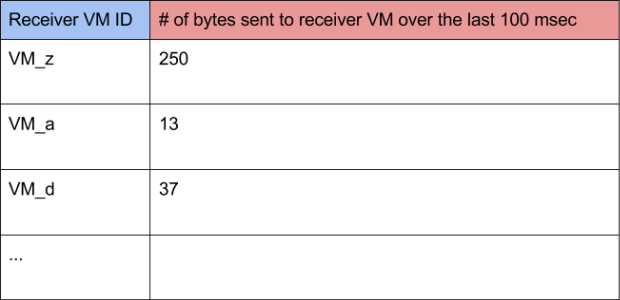
\includegraphics[scale=0.65]{measurement.png}

 \caption{The report data structure for one VM is shown above. Report is an associated array with key, value as follows. key is a VM id that communicated with this VM over the past 100 msec. The associated value is the number of bytes this VM communicated with the VM with id key in the past 100 msec.}

\end{figure}

\FloatBarrier
\LARGE{\textbf{3 Analysis}}

\normalsize

In this section, we’ll look at a few of the common use cases of Placr and how it performs in each.  We’ll be looking at varying levels of occupancy, job size, job arrival rate in the data center, and strategies used by other users.

\Large{\textbf{3.1 Low Number of VMs}}

\normalsize
A job with a low number of VMs is the most basic use case of the system.  In this case, all VMs will be in the same group unless the data center has very low occupancy. Our system should minimize the time taken to complete the job through close placement of VMs. Additionally, since the system shuts down after all VMs are in the same group, it should be cost effective except in the case of very low occupancy.

In the very low occupancy case, Placr will try to keep the VMs distributed in as few groups as possible and in the same cluster.  Unfortunately it will also use two extra VMs until all VMs are in the same group.  If it turns out this not rare, the system will need modifications.

\end{document}



